\chapter{MANIPULATOR DESIGN \& PROTOTYPING}

This chapter presents the comprehensive design, development, and prototyping process of the robotic manipulator system. The development methodology encompasses computer-aided design (CAD) modeling, material selection, component sourcing, assembly procedures, and comprehensive testing protocols.

\section{Requirements and Performance Specifications}

The manipulator design is governed by functional and performance requirements derived from the target application. The system must provide 
sufficient reach and workspace to access targets without frequent base repositioning, offer adequate degrees of freedom for precise positioning
 in constrained environments, and should support standardized interfaces for interchangeable end-effectors.

In addition to these primary objectives, the design process is guided by constraints related to cost, manufacturability, maintainability,
 and operational safety. Requirements are elicited from the target use-case and translated into verifiable performance metrics that can be 
 validated experimentally. Particular emphasis is placed on robustness to environmental disturbances, repeatability under repeated actuation 
 cycles, and energy efficiency given the specified power budget. The specification envelope consequently balances competing objectives
  (payload versus inertia, stiffness versus weight, accuracy versus cost) using a conservative design margin to ensure reliability in field 
  conditions.


\section{Manipulator Architecture and Components}

The manipulator employs a 2-degree-of-freedom (2-DOF) configuration with a base joint (360° range) and a shoulder joint (360° range).
Link design utilizes T-slot 4040 aluminum for the base and shoulder links to achieve an optimal strength-to-weight ratio, reduced inertia, and lower cost, and
3D-printed PLA for joint housings (rapid prototyping). Actuator
selection includes NEMA 17 stepper motors with a 30:1 gear reduction for the base joint and a NEMA 17 stepper motor for the shoulder joint.
The overall kinematic structure is chosen to provide a well-conditioned workspace for the intended task while limiting dynamic coupling
and minimizing reflected inertia at the joints. Material choices follow a mass-stiffness optimization rationale: aluminum members provide
structural rigidity at critical load-bearing links, whereas lightweight 3D-printed PLA housings reduce moving mass, improve acceleration capabilities and
mitigate overshoot. Transmission ratios are selected to trade motor torque amplification against backdrivability and positioning
resolution, with microstepping control improving smoothness at low speeds. The architecture is modular, enabling substitution
of end-effectors and straightforward integration of alternative sensors (e.g., force/torque or proximity) without modifications 
to the primary structure.

\subsection*{Kinematic parameters and workspace}
For analysis and control, the arm is modeled as a planar 2-DOF serial chain with revolute joints. The link lengths are
\(L_1 = 0.25\,\mathrm{m}\) and \(L_2 = 0.25\,\mathrm{m}\). The nominal planar reach measured from the base frame to the tool tip therefore spans the annulus
\([\,|L_1-L_2|,\; L_1+L_2\,] = [\,0.00\,\mathrm{m},\; 0.50\,\mathrm{m}\,]\), neglecting self-collisions and end-effector offsets.

The standard Denavit--Hartenberg (DH) parameters used to formulate forward and inverse kinematics are summarized in Table~\ref{tab:dh_params}.

\begin{table}[H]
\centering
\caption{DH parameters for the 2-DOF planar manipulator (standard convention).}
\label{tab:dh_params}
\begin{tabular}{|c|c|c|c|c|}
\hline
Joint $i$ & $a_i$ [m] & $\alpha_i$ [rad] & $d_i$ [m] & $\theta_i$ [rad] \\
\hline
1 & 0.25 & 0 & 0 & $\theta_1$ \\
2 & 0.25 & 0 & 0 & $\theta_2$ \\
\hline
\end{tabular}
\end{table}

\subsection*{Joint limits and reachable sector}
Unless otherwise constrained, both joints operate over approximately \([-180^{\circ},\,180^{\circ}]\). Table~\ref{tab:joint_limits} summarizes the limits used during testing. With these limits the end-effector can sweep a full circle about the base within the annular workspace described above; additional fixtures or cable routing may further restrict the usable sector during operation.

\begin{table}[H]
\centering
\caption{Joint limits used for analysis and testing.}
\label{tab:joint_limits}
\begin{tabular}{|c|c|c|}
\hline
Joint & Lower limit [deg] & Upper limit [deg] \\
\hline
Base (\(\theta_1\)) & -180 & 180 \\
Shoulder (\(\theta_2\)) & -180 & 180 \\
\hline
\end{tabular}
\end{table}

\section{Electrical System Design}

The system architecture includes a 12\,V DC main power supply (5\,A capacity). The control architecture features two Arduino Nano microcontrollers,
A4988 stepper motor drivers with microstepping capability, USB and wireless communication interfaces, and comprehensive 
safety systems including emergency stop, limit switches, and current monitoring. Wiring employs shielded cables for signal integrity,
strain relief and cable guides for mechanical protection, color-coded wiring for identification, and modular connectors for easy disassembly.

\begin{figure}[H]
\centering
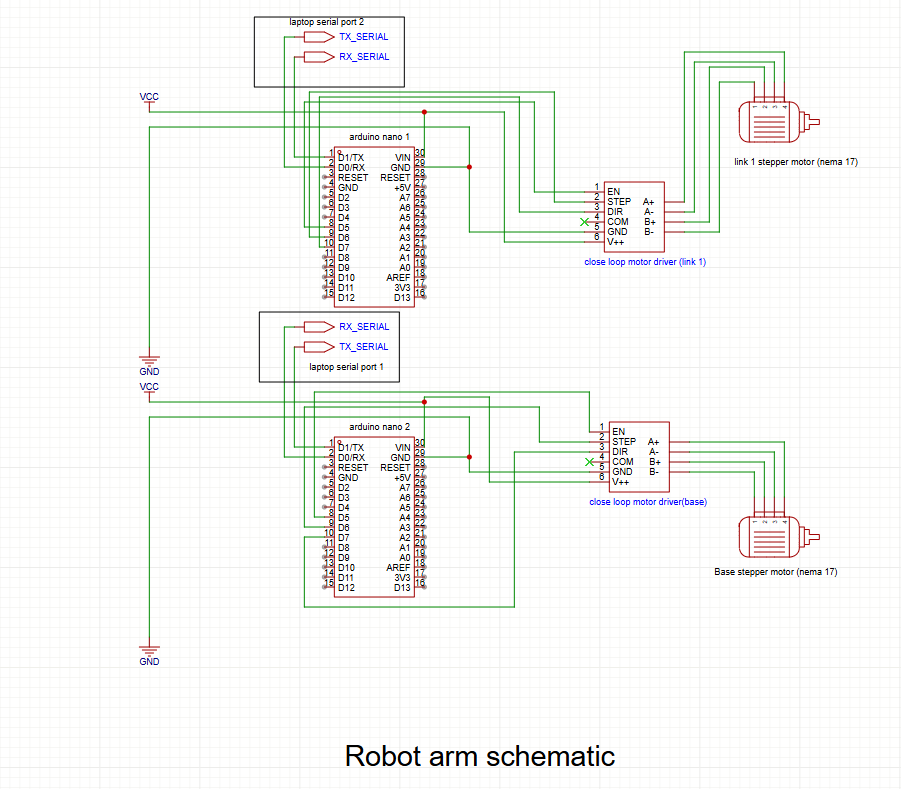
\includegraphics[width=0.95\linewidth]{pictures/arm_schamatic.png}
\caption{Electrical schematic of the robot arm control system, showing controller, drivers, and power distribution.}
\label{fig:arm_schematic}
\end{figure}

Two Arduino Nano microcontrollers implement a distributed control architecture. An on-board voltage regulator is used to regulate the supply to 
5\,V for the Arduino Nano. Each board receives joint-level position commands for its
assigned link via an independent serial interface and performs local trajectory generation, thereby decoupling the control loops for the base 
and shoulder. For the base joint, the software accounts for an effective transmission ratio of 30:1 when converting commanded angles to motor 
steps and velocity profiles.

Both actuators are driven by stepper motor drivers with microstepping to enhance positioning accuracy and disturbance rejection. The controllers 
interface with the microcontrollers using standard ENABLE, STEP, and DIRECTION control signals (as wired in Fig.~\ref{fig:arm_schematic}). The 
drivers commutate the motor phases by switching the A$+$, A$-$, B$+$, and B$-$ outputs; the polarity is governed by the DIRECTION input while 
incremental motion is effected by STEP pulses. Microstepping is employed to achieve smoother motion and increased effective resolution.


\section{Bill of Materials}

The bill of materials enumerates key mechanical and electrical components that satisfy the derived specifications while maintaining
 availability from multiple vendors. Selection criteria include performance-to-cost ratio, durability, interoperability with standard 
 interfaces, and lead time. Table~\ref{tab:components_bom} summarizes representative components used in the prototype.

\begin{table}[H]
\centering
\caption{Bill of materials for the manipulator prototype.}
\label{tab:components_bom}
\begin{tabular}{|p{0.28\linewidth}|c|p{0.30\linewidth}|p{0.30\linewidth}|}
\hline
Item & Qty & Specification & Function \\
\hline
T-slot aluminum extrusion & 2 & 4040 profile & Primary structural members \\
Harmonic drive & 1 & 30 to 1 gear reduction & Torque amplification \\
Stepper motor & 2 & NEMA 17, 1.8 deg/step & Joint actuation \\
Stepper driver & 2 & ENABLE/STEP/DIR inputs & Motor control \\
Microcontroller & 2 & Arduino Nano & Control and communication \\
Power supply & 1 & 12V, 5A & DC power source \\
Shielded cable & - & Twisted-pair & Wiring harness \\
3D printing filament (PLA) & 1 & 1 kg spool, 1.75 mm & Rapid prototyping of non-load parts \\
3D printing filament (PLA) & 1 & 1 kg spool, 1.75 mm & Durable housings and brackets \\
\hline
\end{tabular}
\end{table}


\section{Fabrication and Assembly}
Manufacturing methods include CNC machining for aluminum components (precision and durability), 3D printing for PLA plastic housings and brackets, manual assembly for component integration and cable routing, and calibration procedures for joint alignment and sensor setup. Dimensional tolerances are specified for bearing seats, pulley alignment, and shaft interfaces to ensure minimal backlash and consistent transmission efficiency. Quality control inspections are performed after each major operation, including visual inspection, dimensional verification with calipers/gauges, and rotational smoothness checks of assembled joints. All project CAD files referenced in this chapter are provided in Appendix~A for completeness and reproducibility.

\begin{figure}[H]
\centering
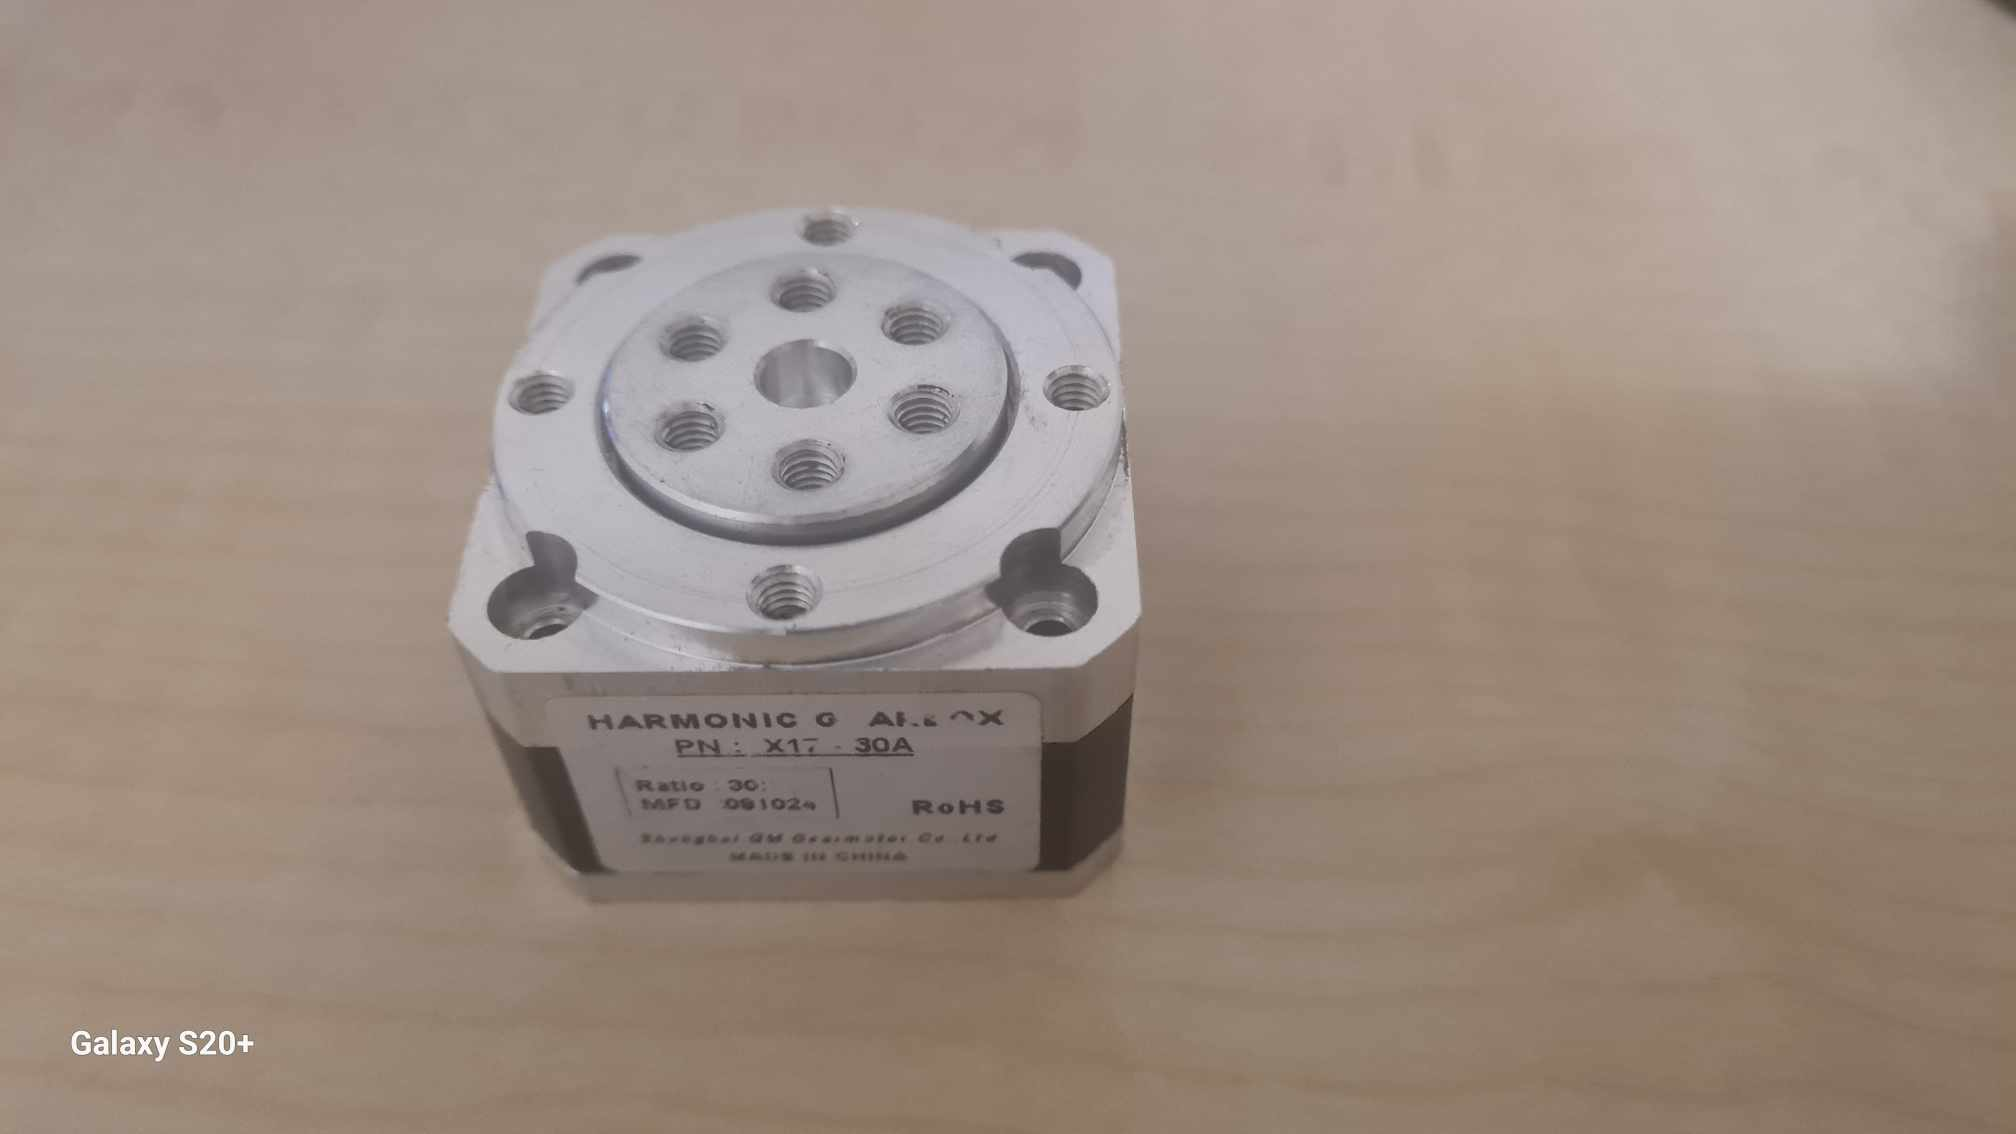
\includegraphics[width=0.48\linewidth]{pictures/gearreducer.jpg}\hfill
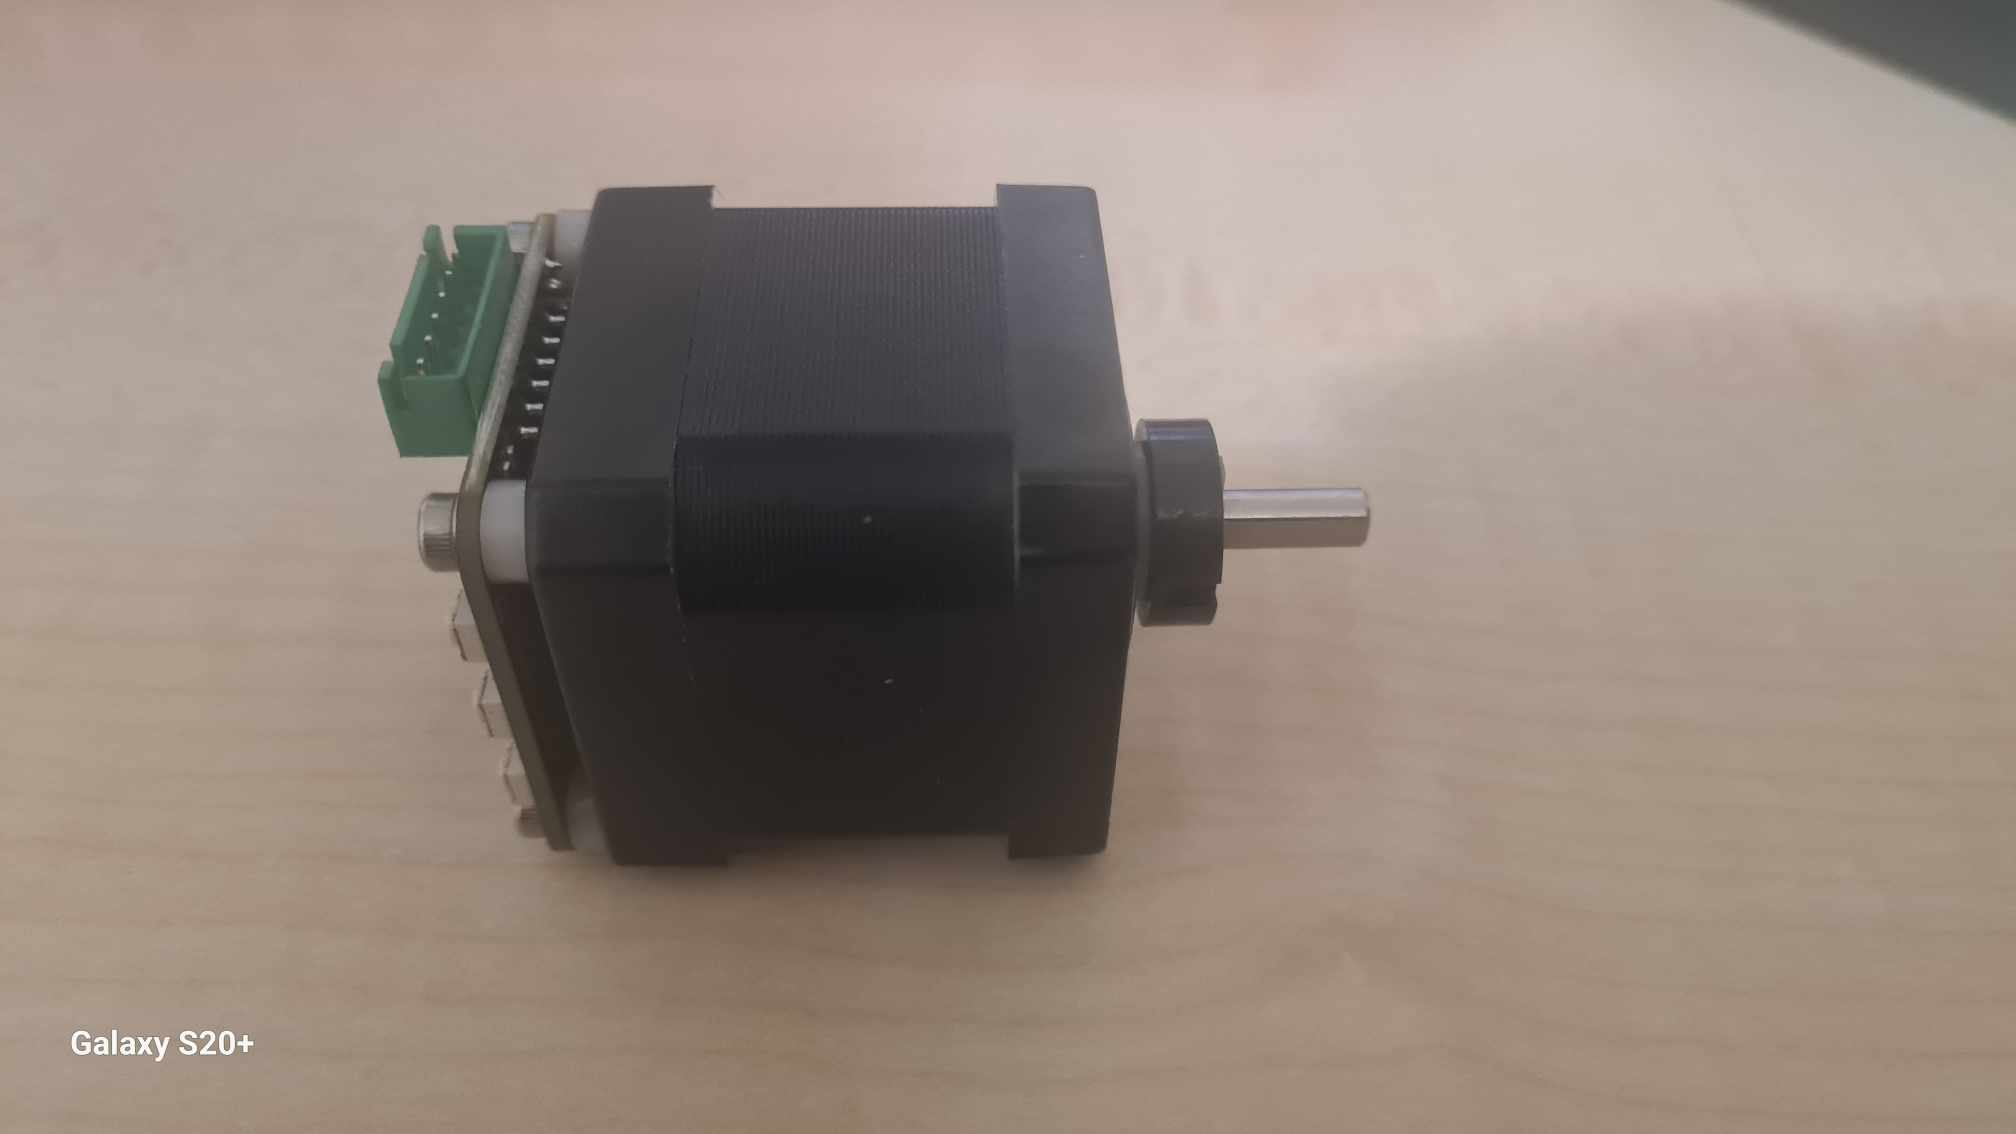
\includegraphics[width=0.48\linewidth]{pictures/nema17.jpg}
\caption{Prototype actuation hardware. Left: compact harmonic-drive gear reducer (30:1) used on the base joint to increase output torque and stiffness while maintaining low backlash. Right: NEMA 17 stepper motor (1.8 deg/step) employed for joint actuation, interfaced via ENABLE/STEP/DIR signals to the driver.}
\label{fig:actuator_photos}
\end{figure}

\begin{figure}[H]
\centering
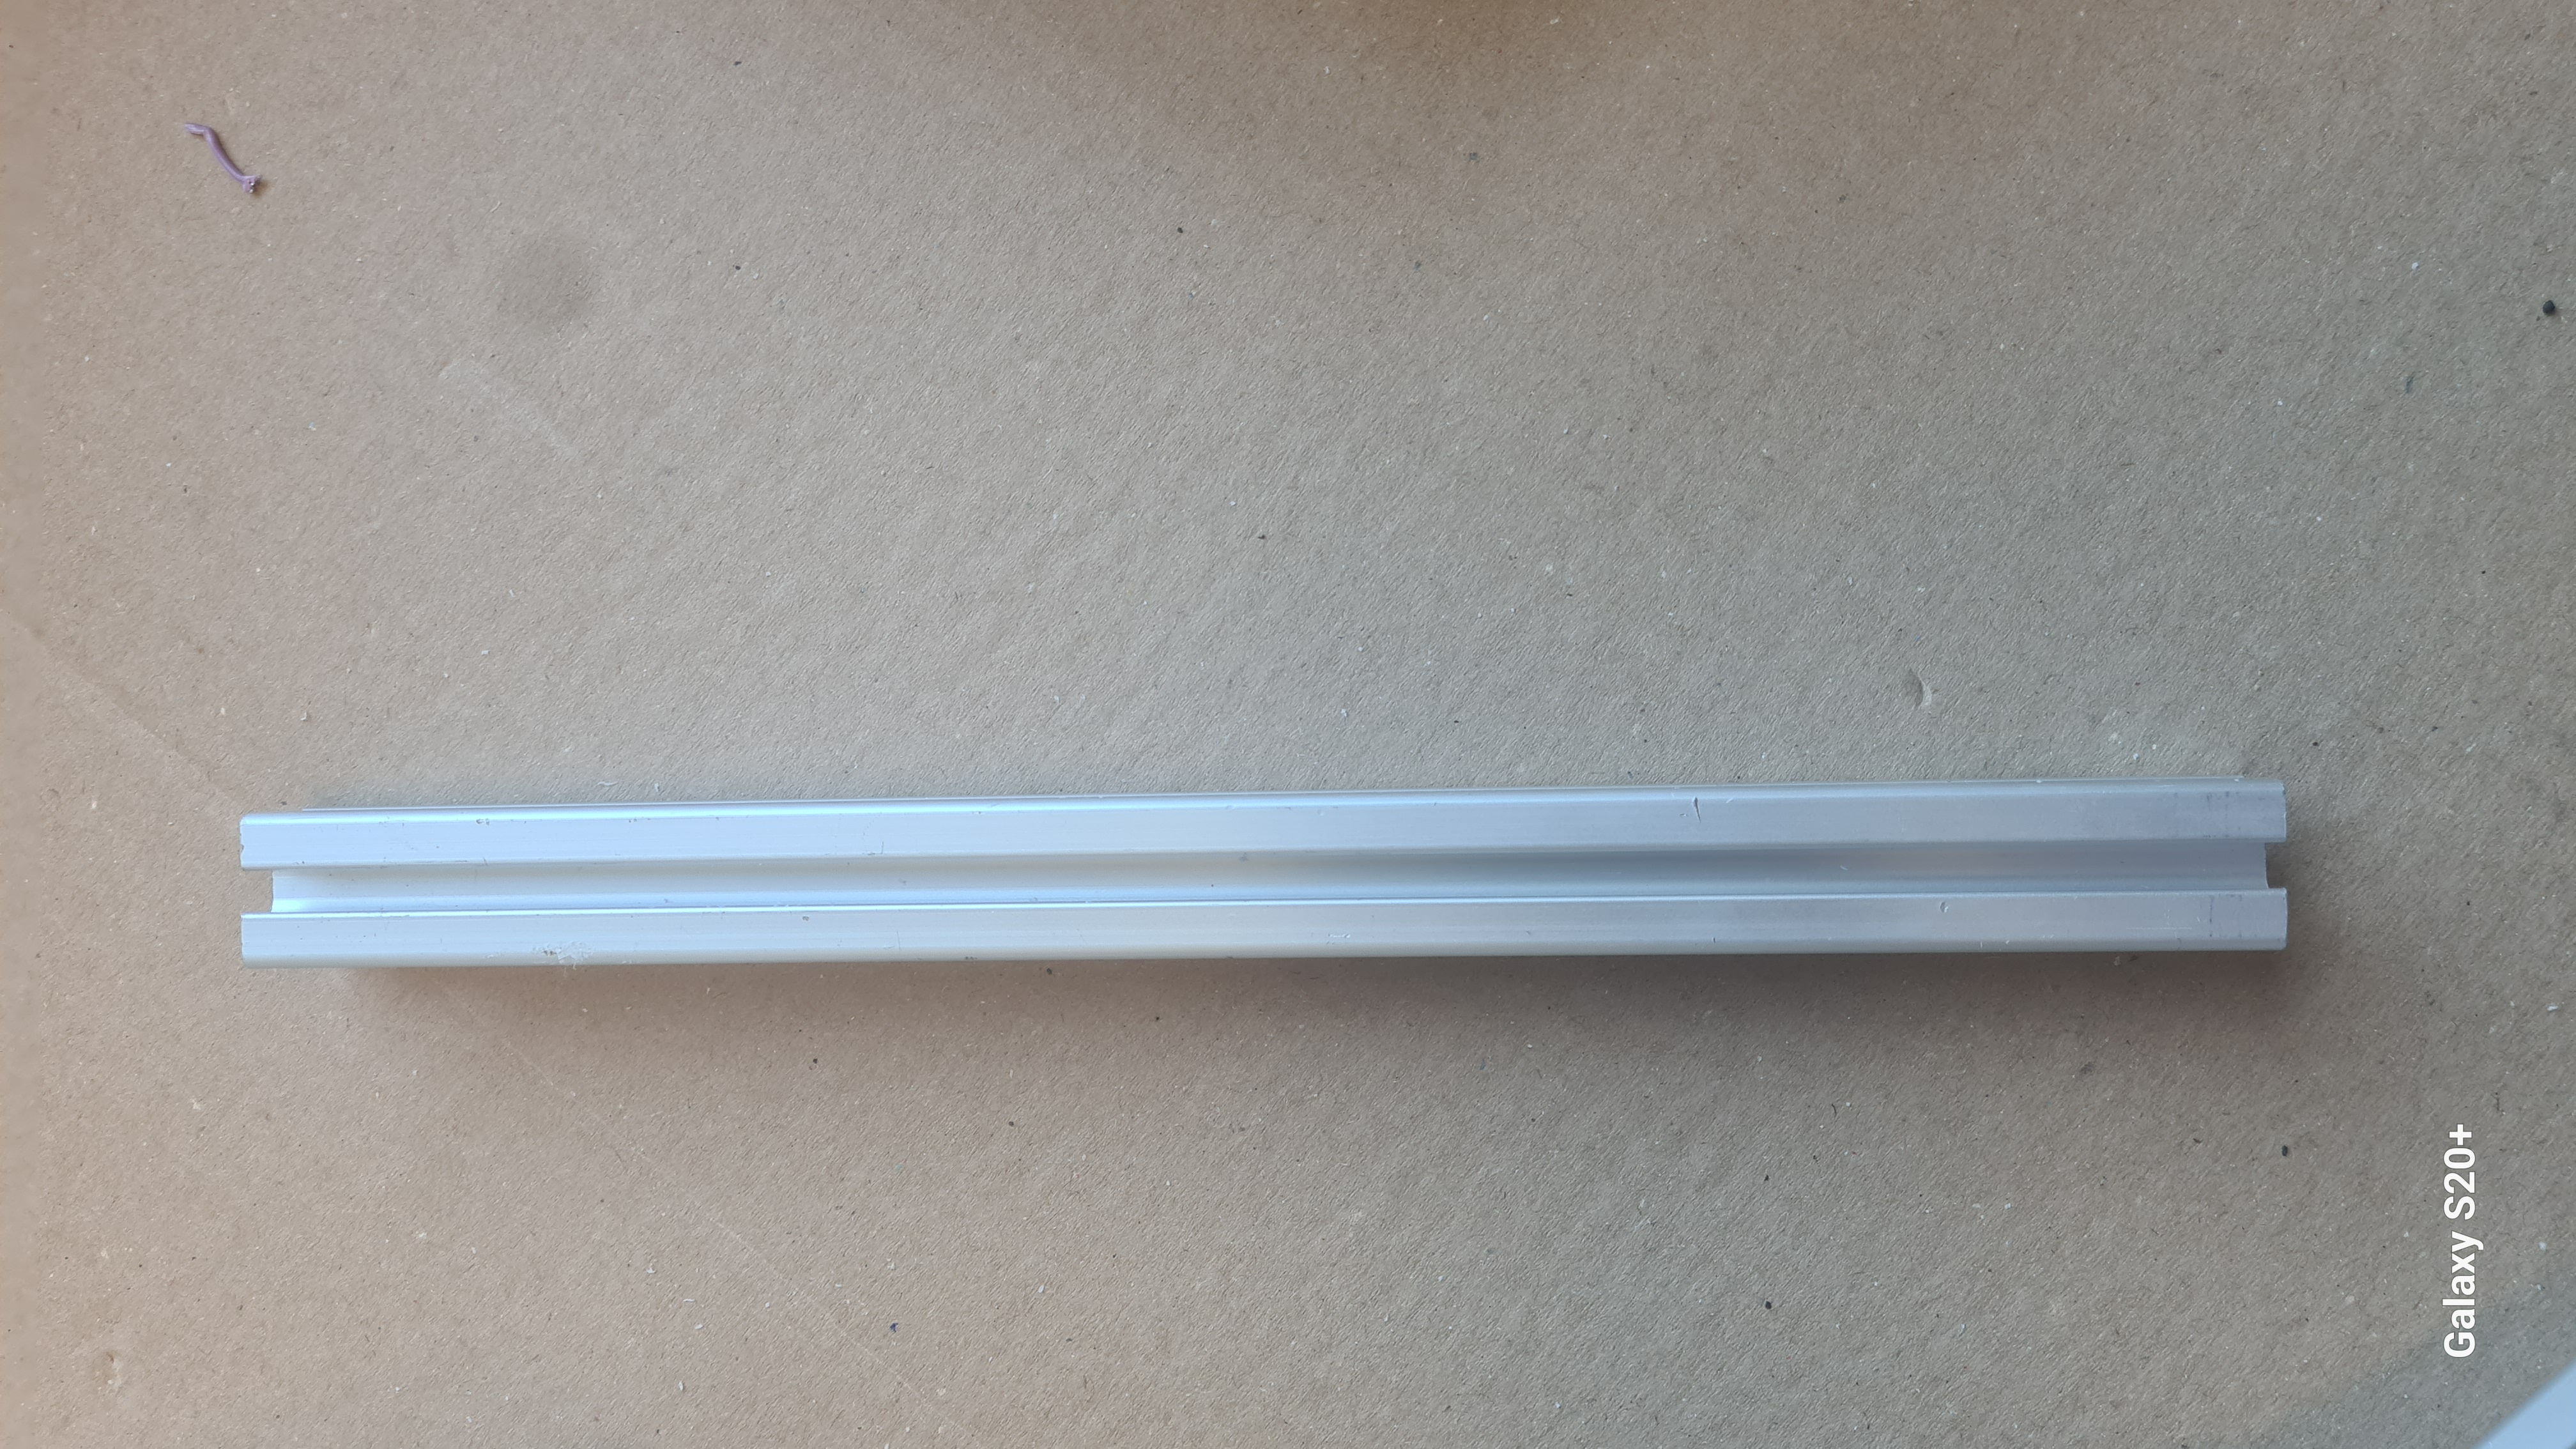
\includegraphics[width=0.48\linewidth]{\detokenize{pictures/ROD LINK.jpg}}\hfill
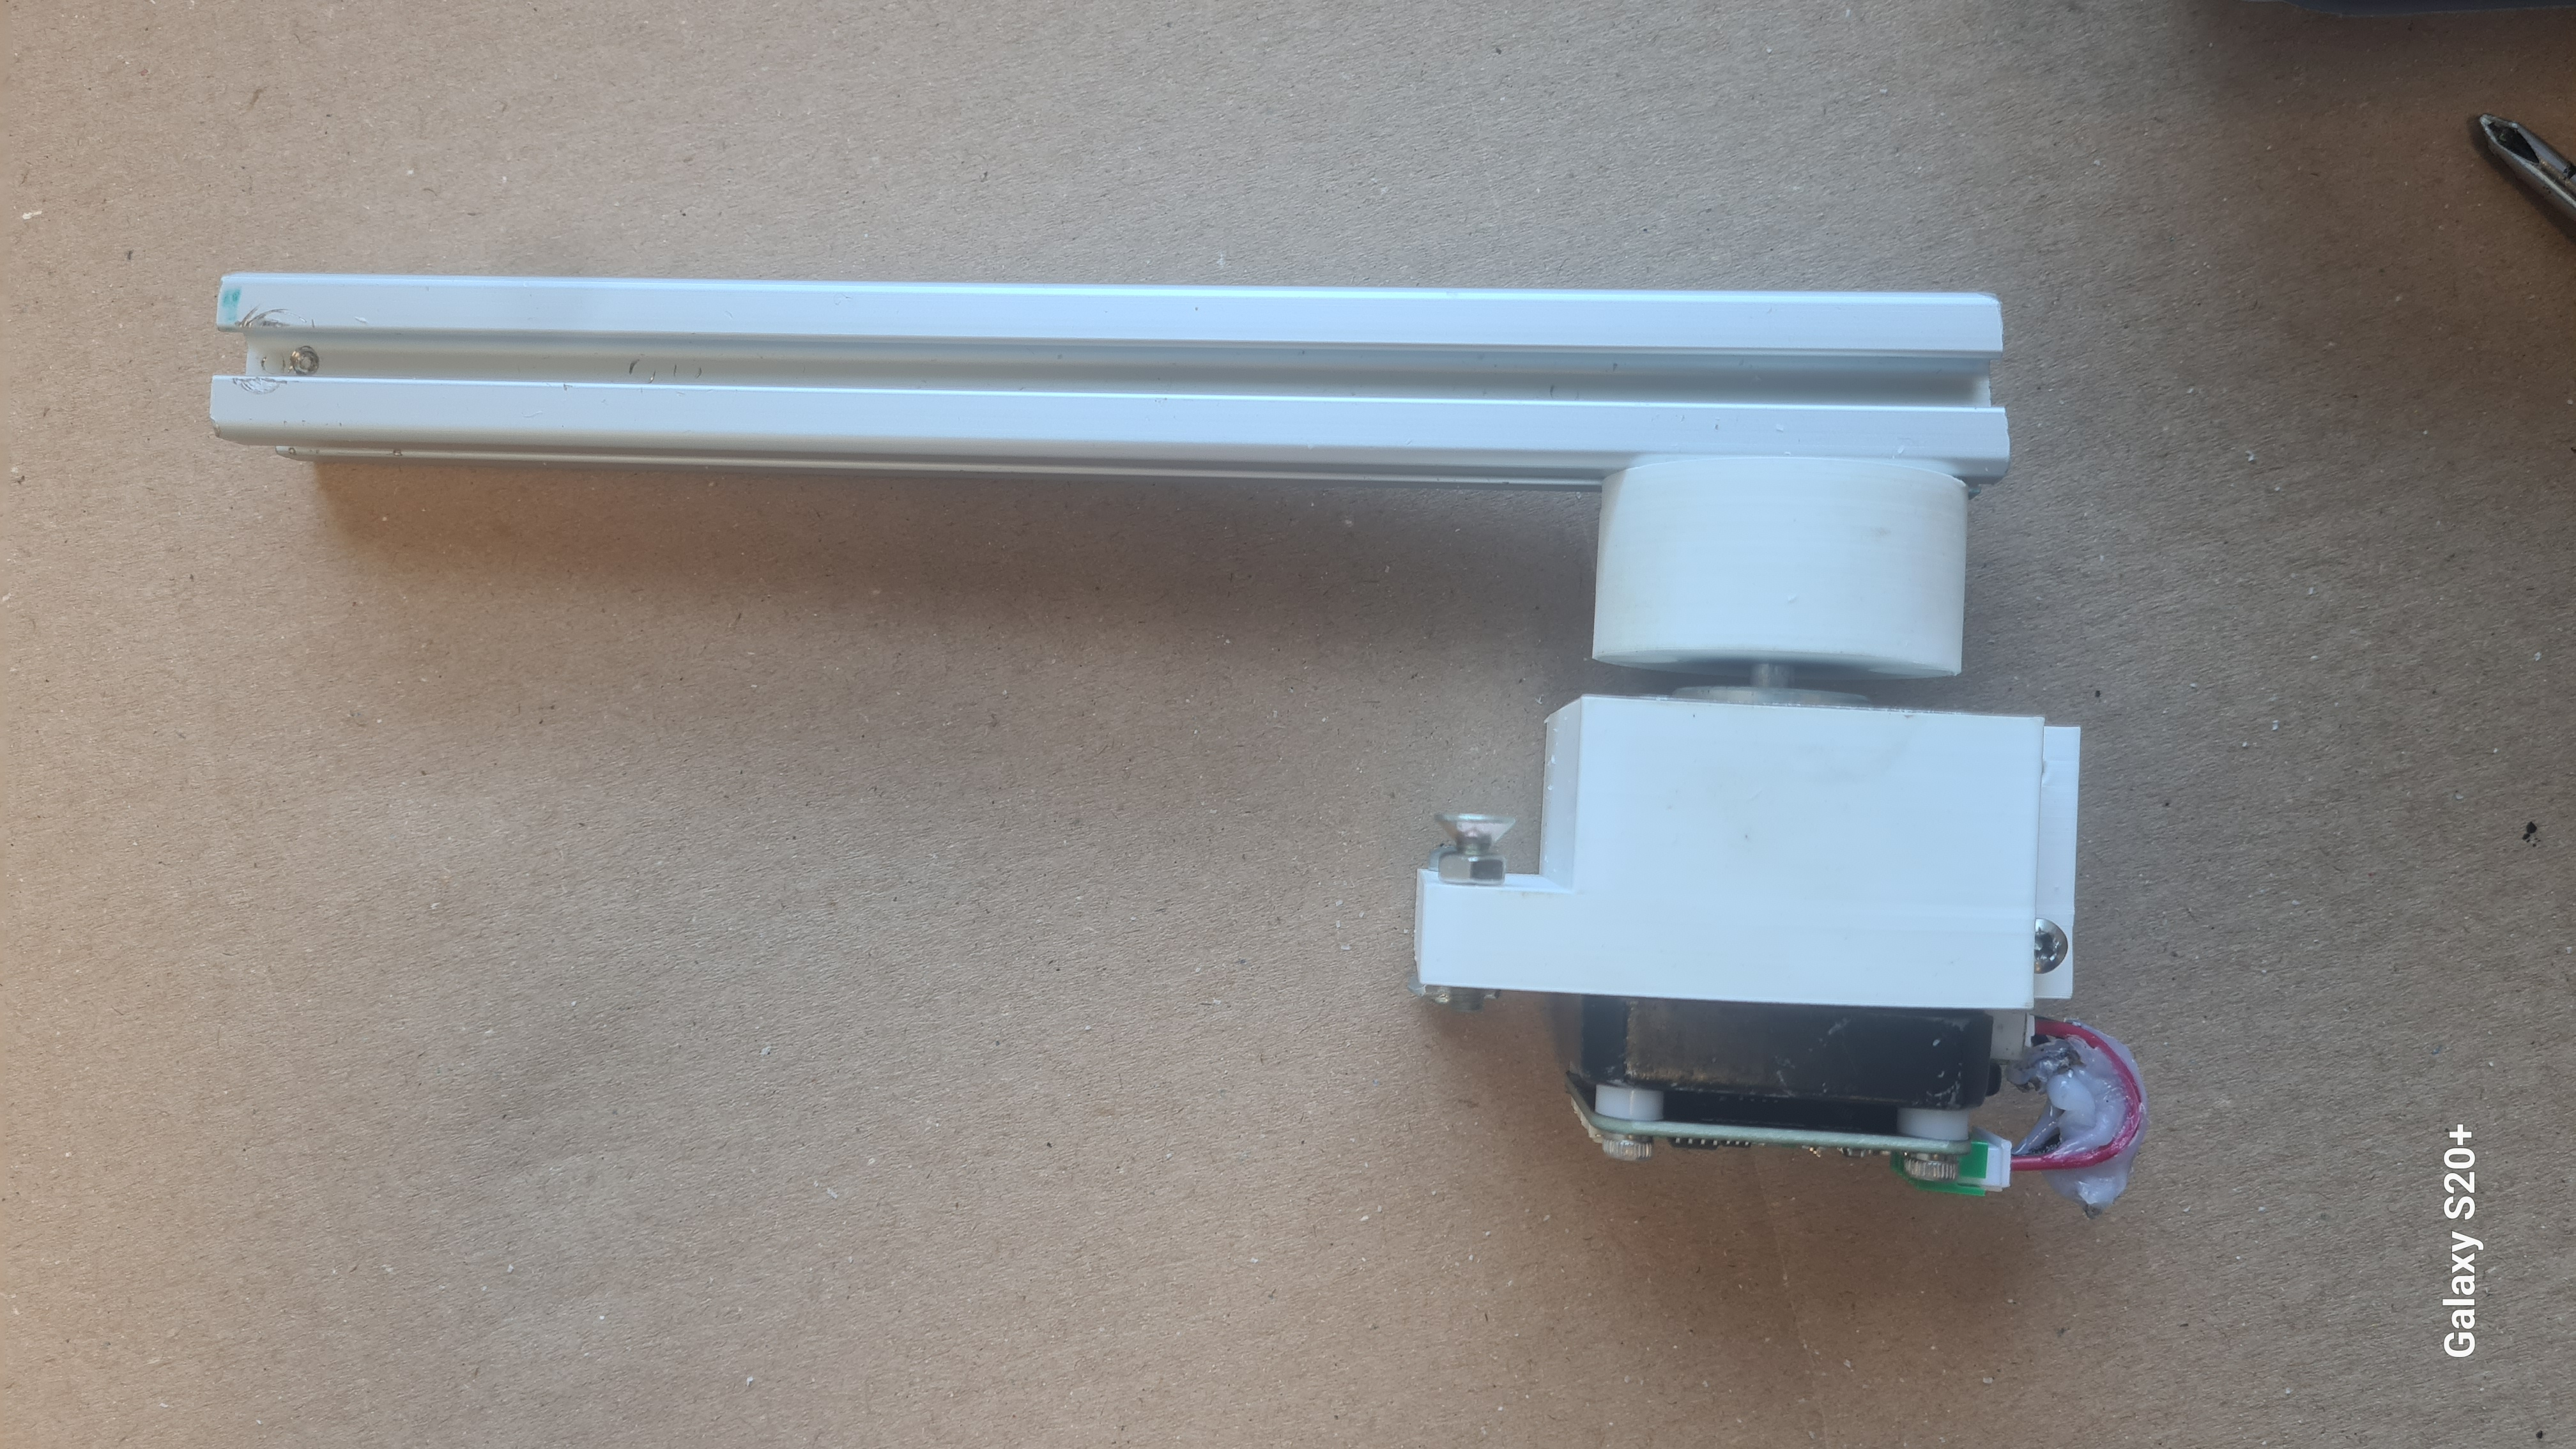
\includegraphics[width=0.48\linewidth]{\detokenize{pictures/shoulder assemble.jpg}}
\caption{Mechanical subassemblies. Left: machined aluminum rod link with T-slot profile used for lightweight, modular link construction. Right: shoulder assembly showing the link interface, printed mount, and fastener pattern enabling quick reconfiguration.}
\label{fig:link_and_shoulder}
\end{figure}

\begin{figure}[H]
\centering
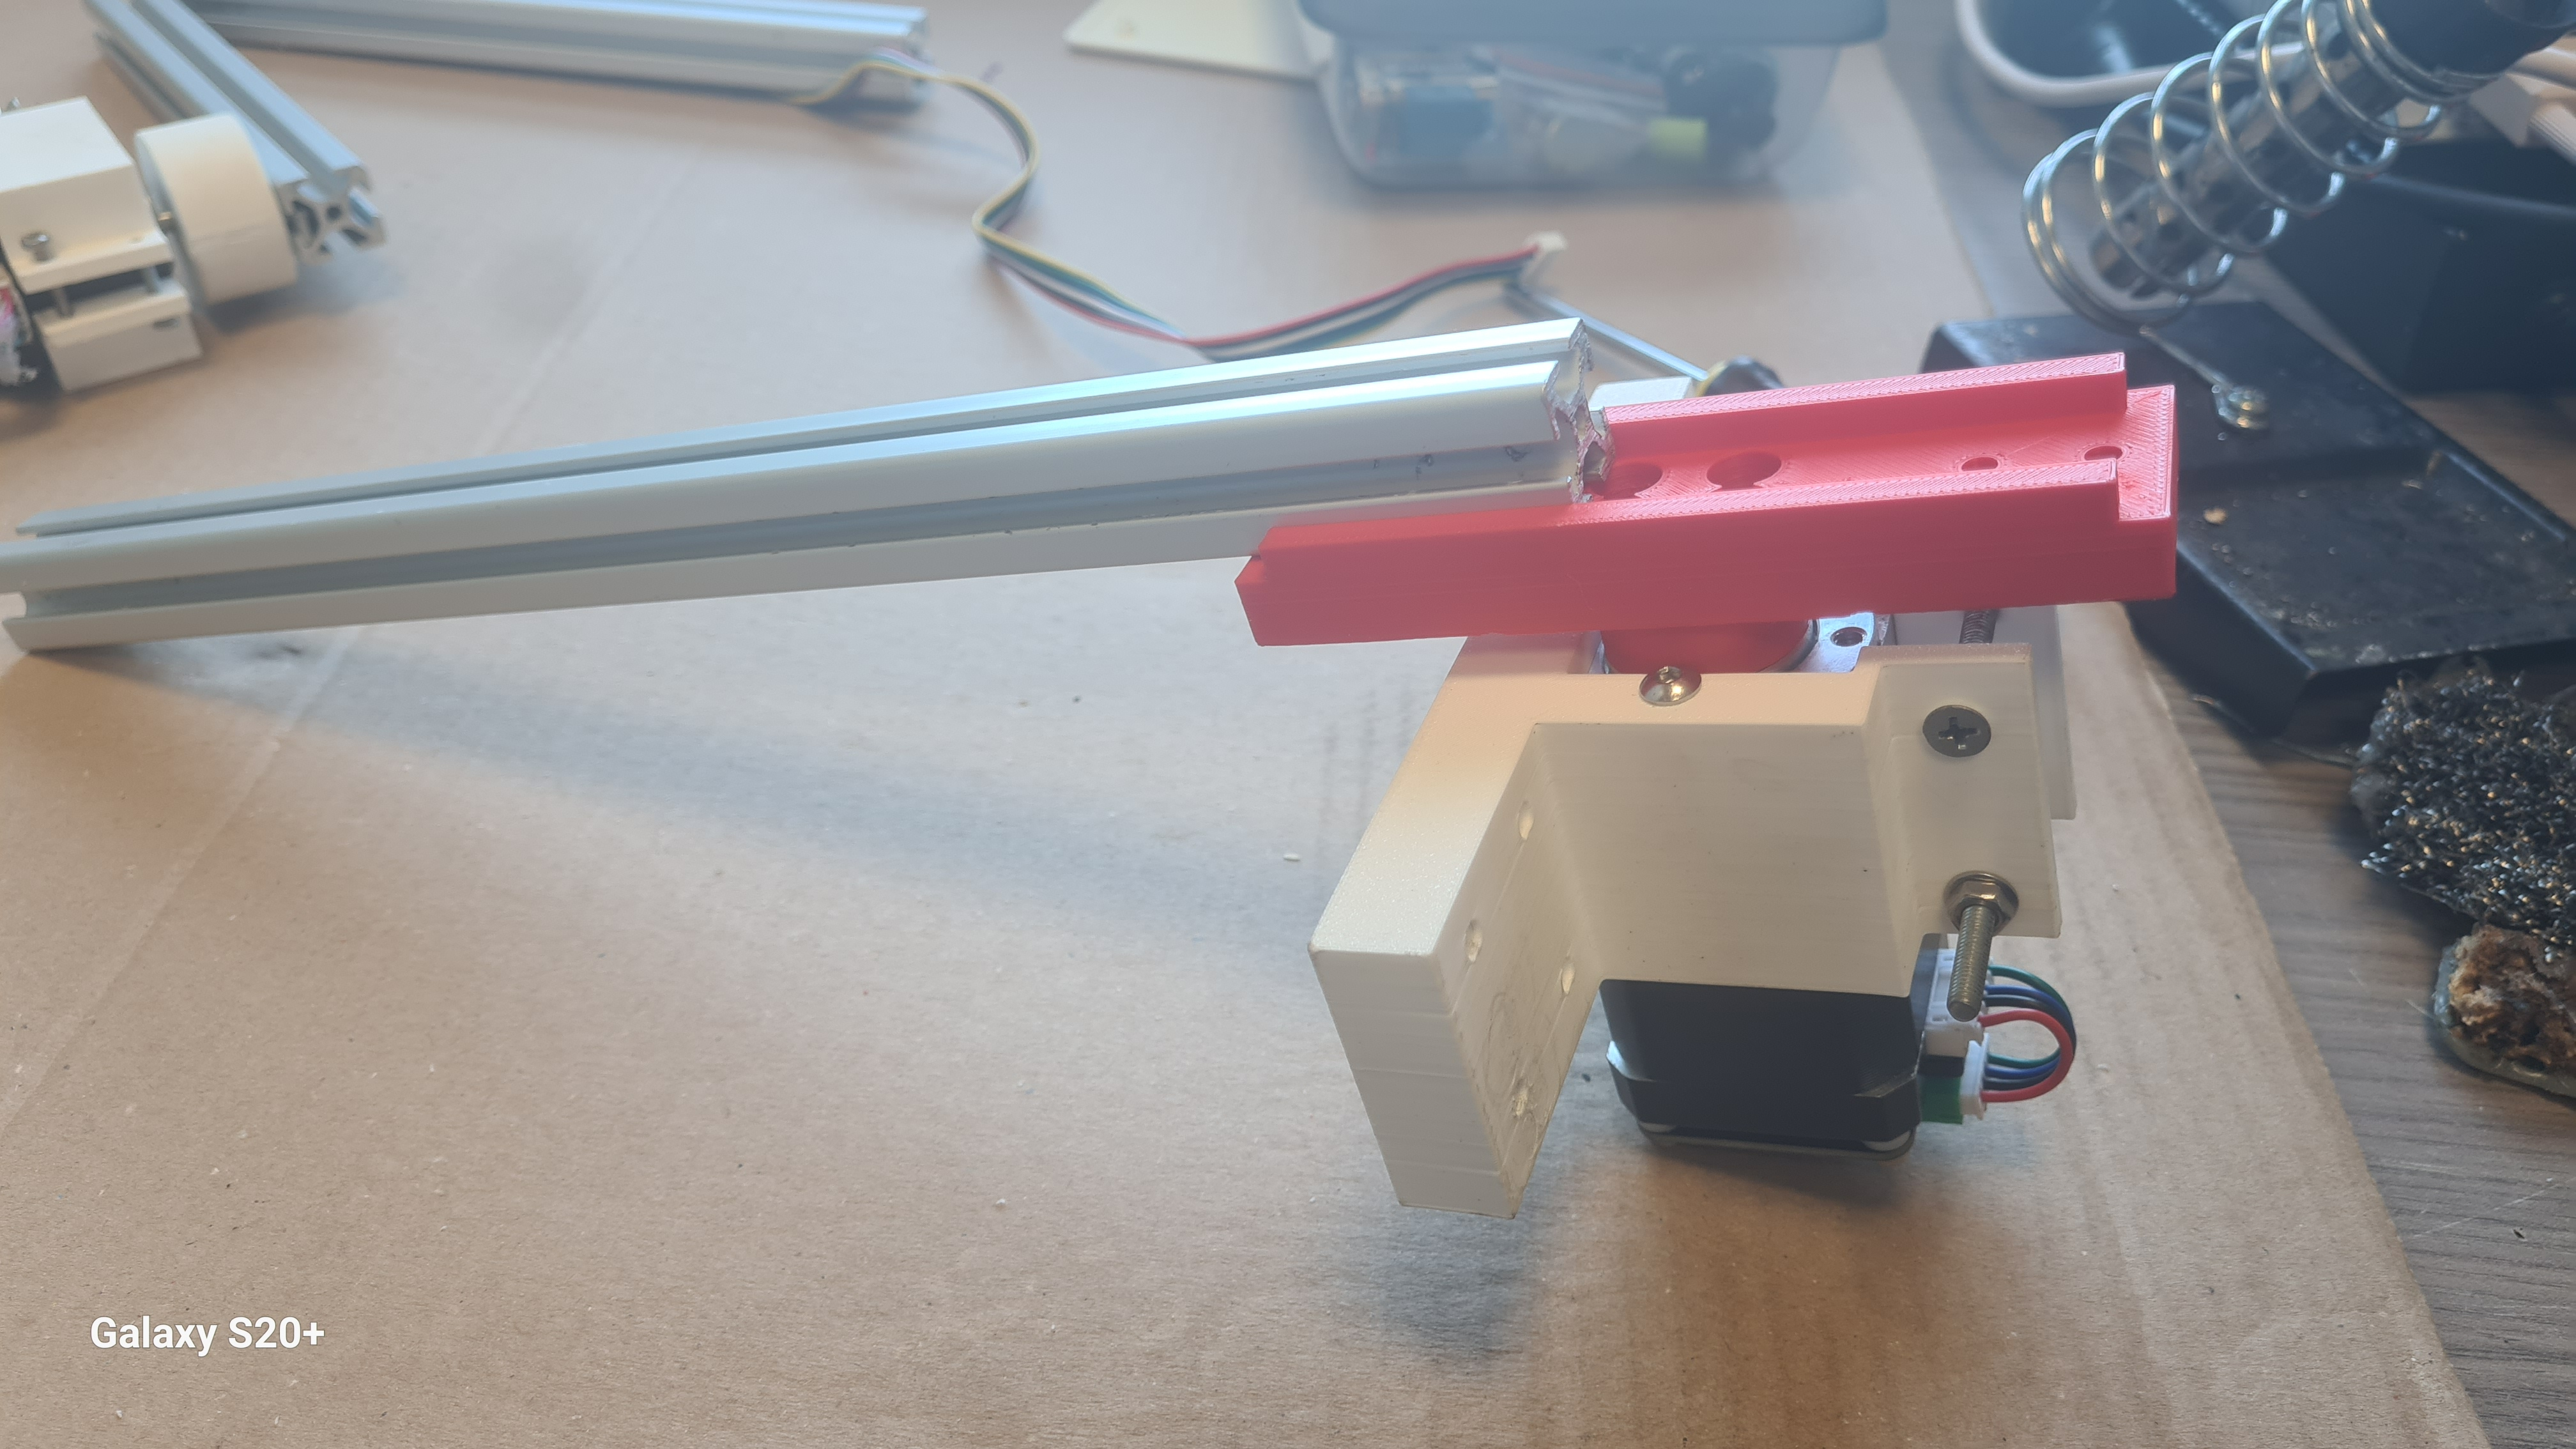
\includegraphics[width=0.48\linewidth]{\detokenize{pictures/BASE JOINT ASSEMBLE.jpg}}\hfill
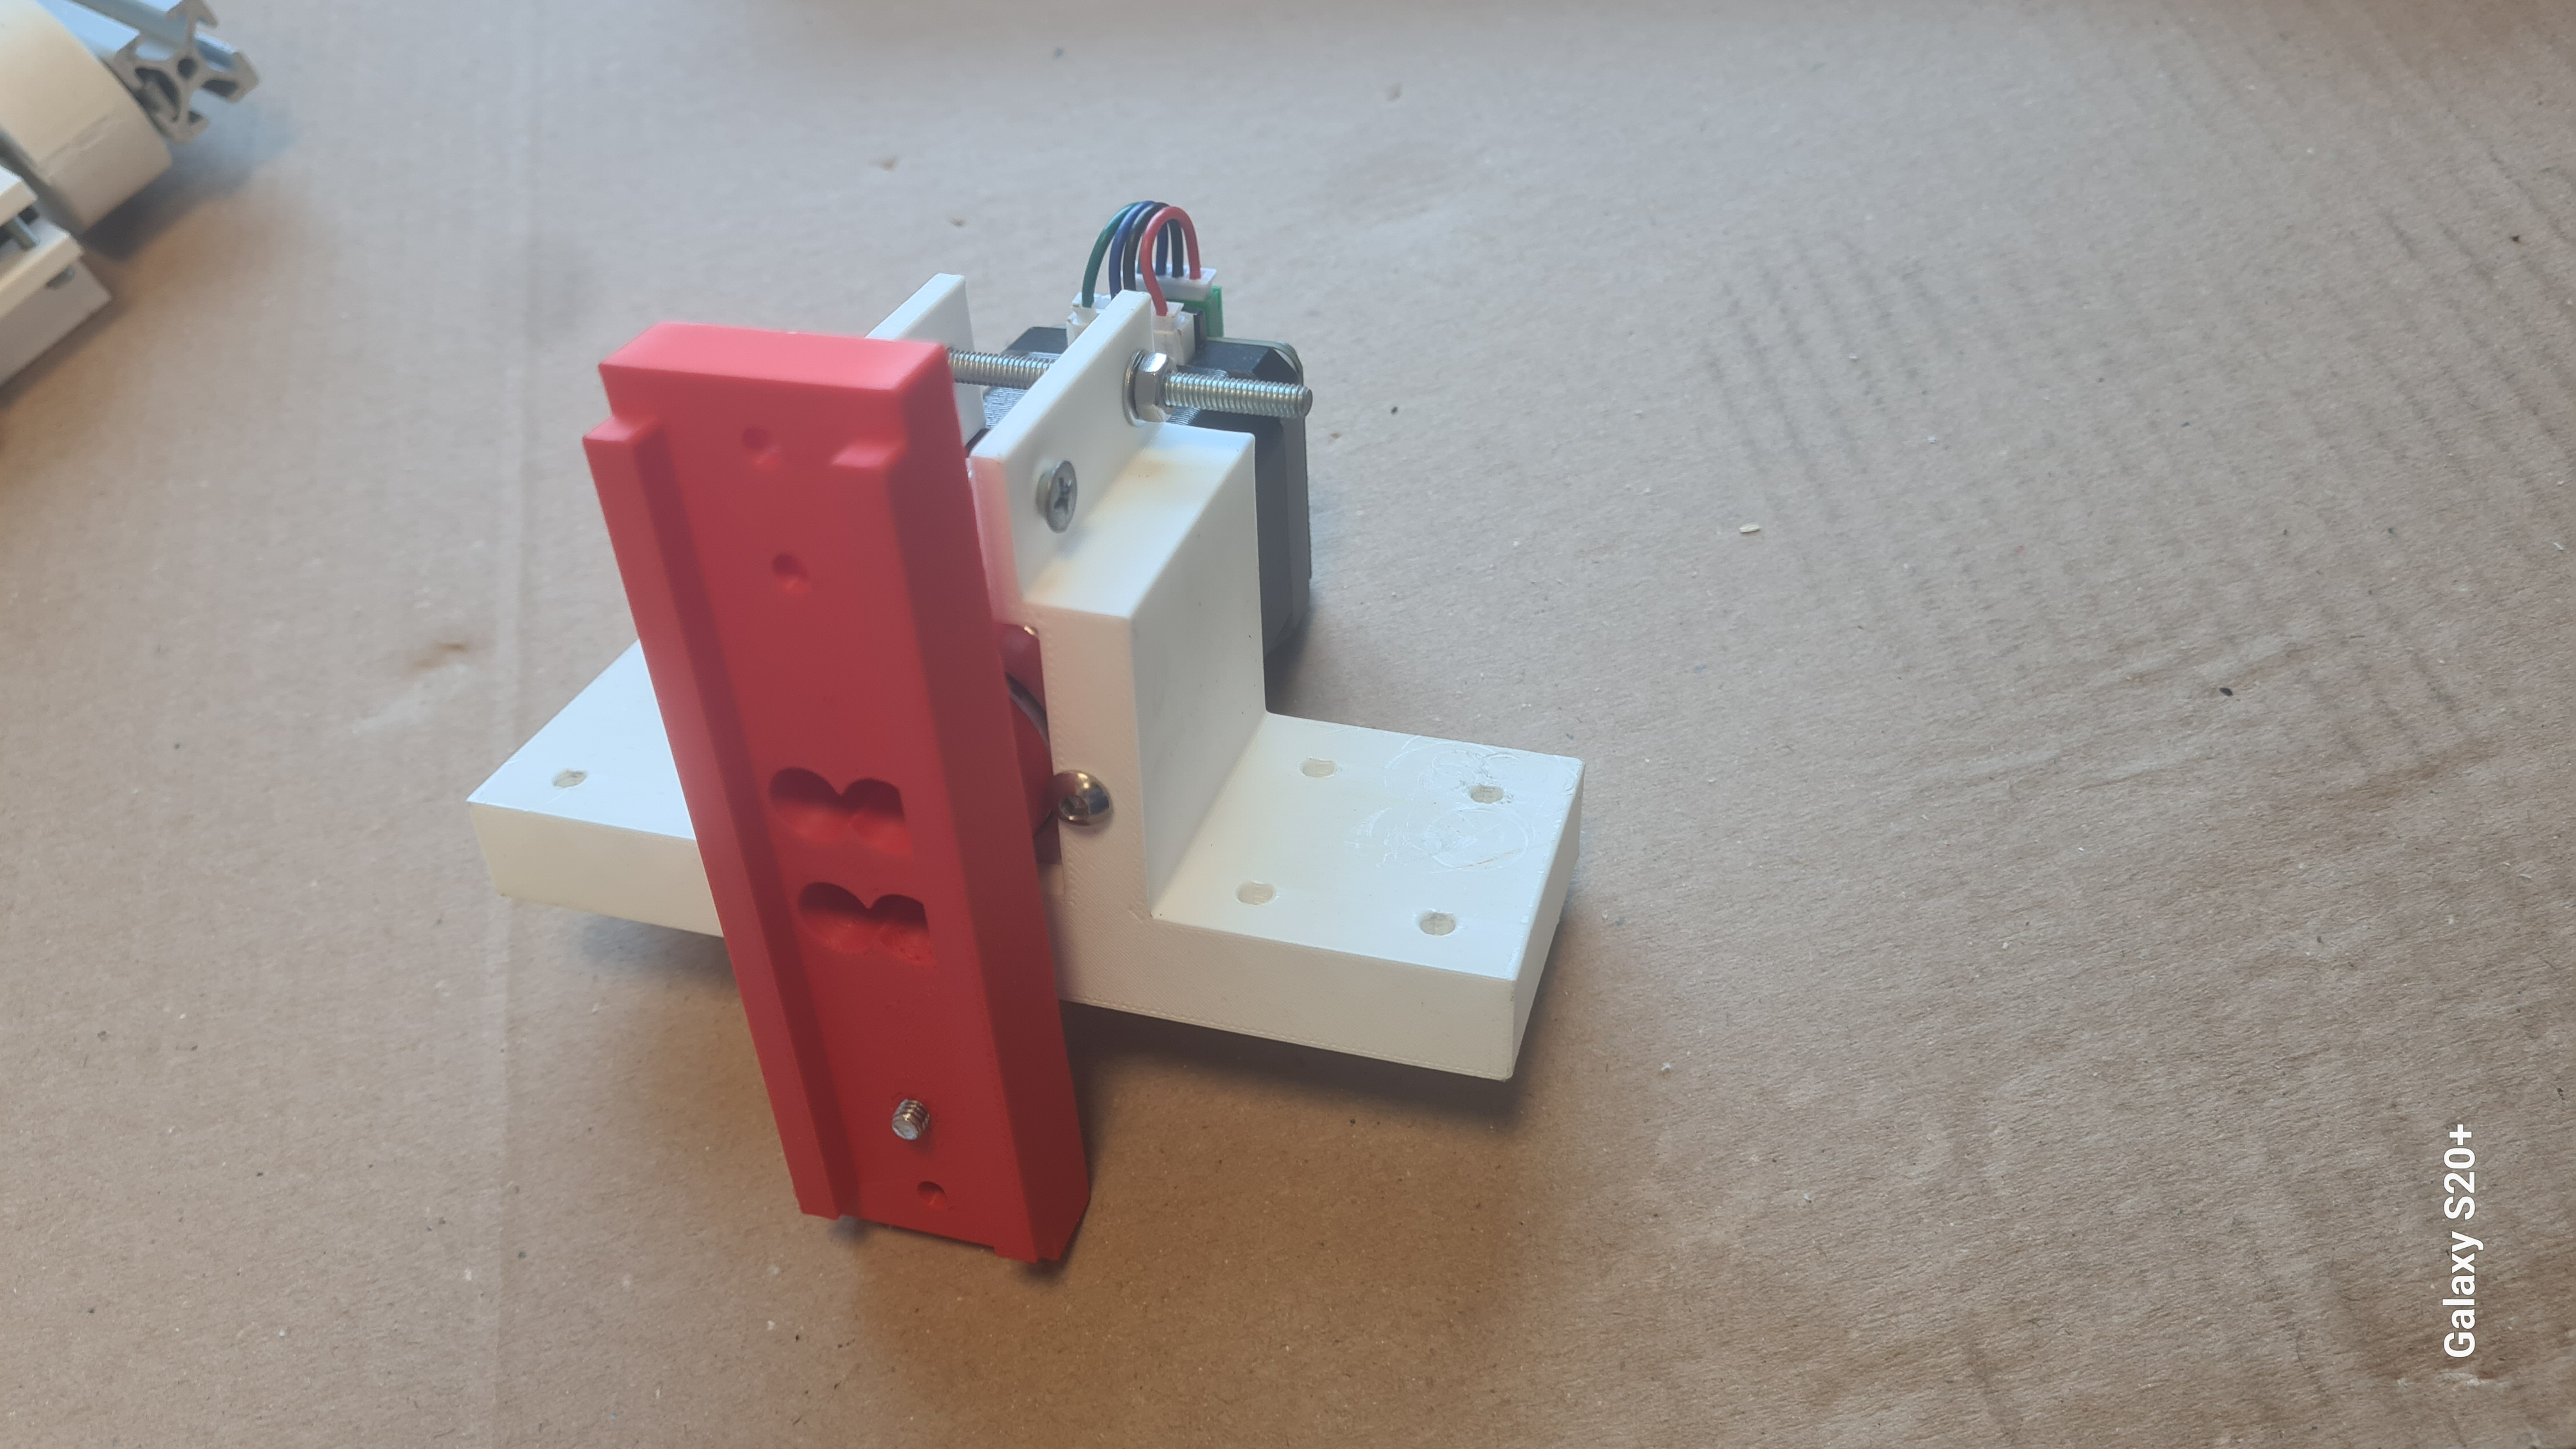
\includegraphics[width=0.48\linewidth]{\detokenize{pictures/BASE JOINT HOLDER.jpg}}
\caption{Base joint details. Left: assembled base joint integrating the gear reducer, stepper motor, and printed housing. Right: base-joint holder bracket that constrains the reducer and provides the structural interface to the frame.}
\label{fig:base_joint_details}
\end{figure}

\begin{figure}[H]
\centering
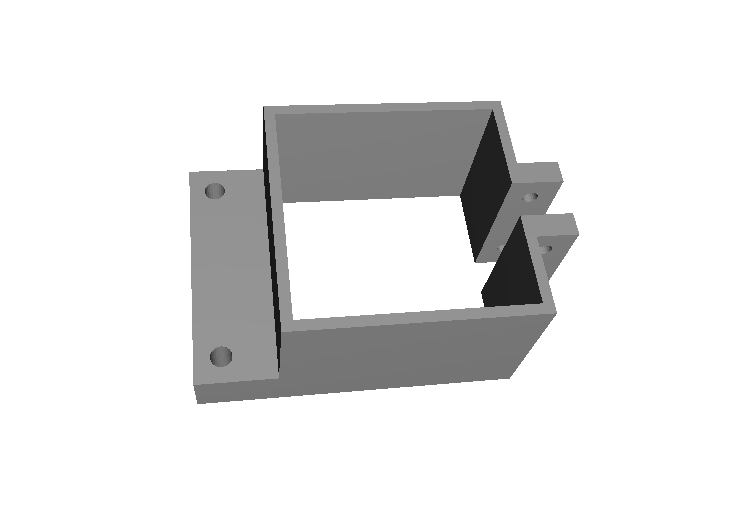
\includegraphics[width=0.48\linewidth]{\detokenize{pictures/stepper holder.png}}\hfill
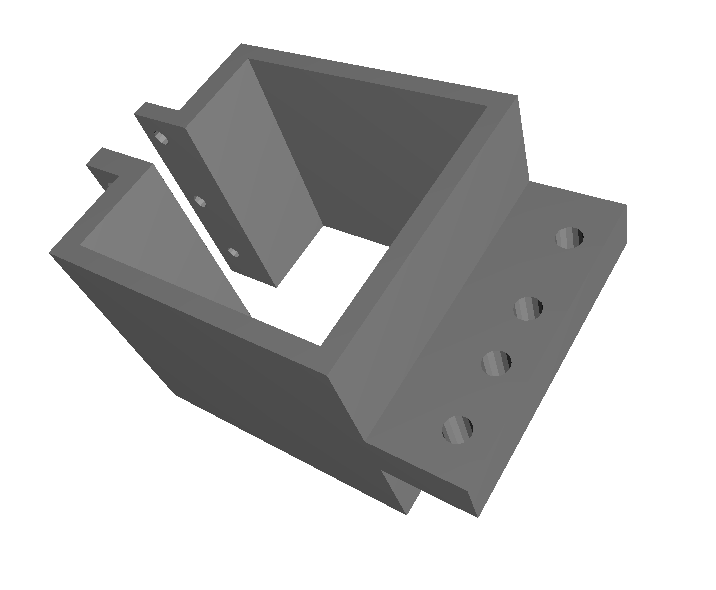
\includegraphics[width=0.48\linewidth]{\detokenize{pictures/stepperHolder.png}}
\caption{CAD snapshots of the stepper holder variants. Left: compact stepper holder with mounting flange for the NEMA 17 frame. Right: reinforced holder variant with additional fastener pattern for increased stiffness and alignment repeatability.}
\label{fig:stepper_holders}
\end{figure}

\begin{figure}[H]
\centering
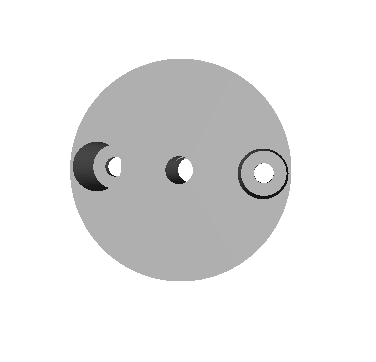
\includegraphics[width=0.48\linewidth]{\detokenize{pictures/shaft connector.png}}\hfill
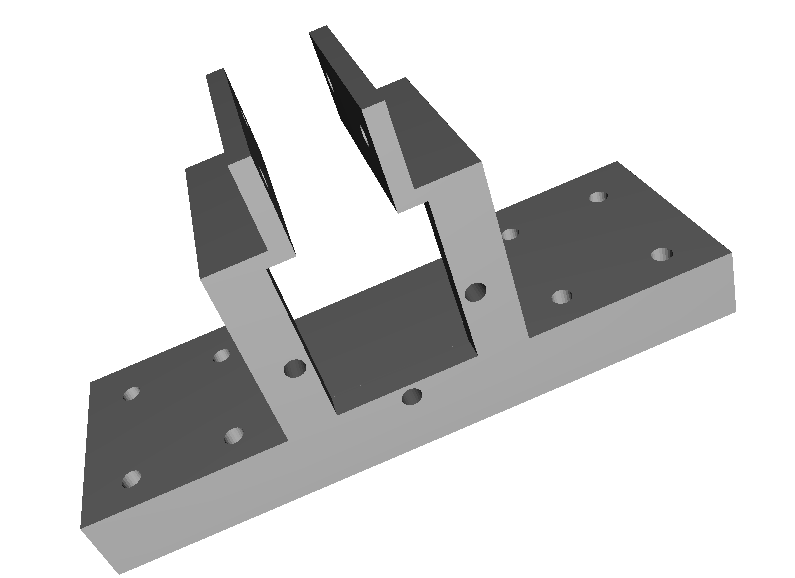
\includegraphics[width=0.48\linewidth]{\detokenize{pictures/base stepper holder.png}}
\caption{Additional CAD components. Left: shaft connector used to couple the stepper shaft to the reducer input while preserving concentricity. Right: base stepper holder showing the through-holes and counterbores that interface to the frame and allow cable clearance.}
\label{fig:connector_and_baseholder}
\end{figure}

\begin{figure}[H]
\centering
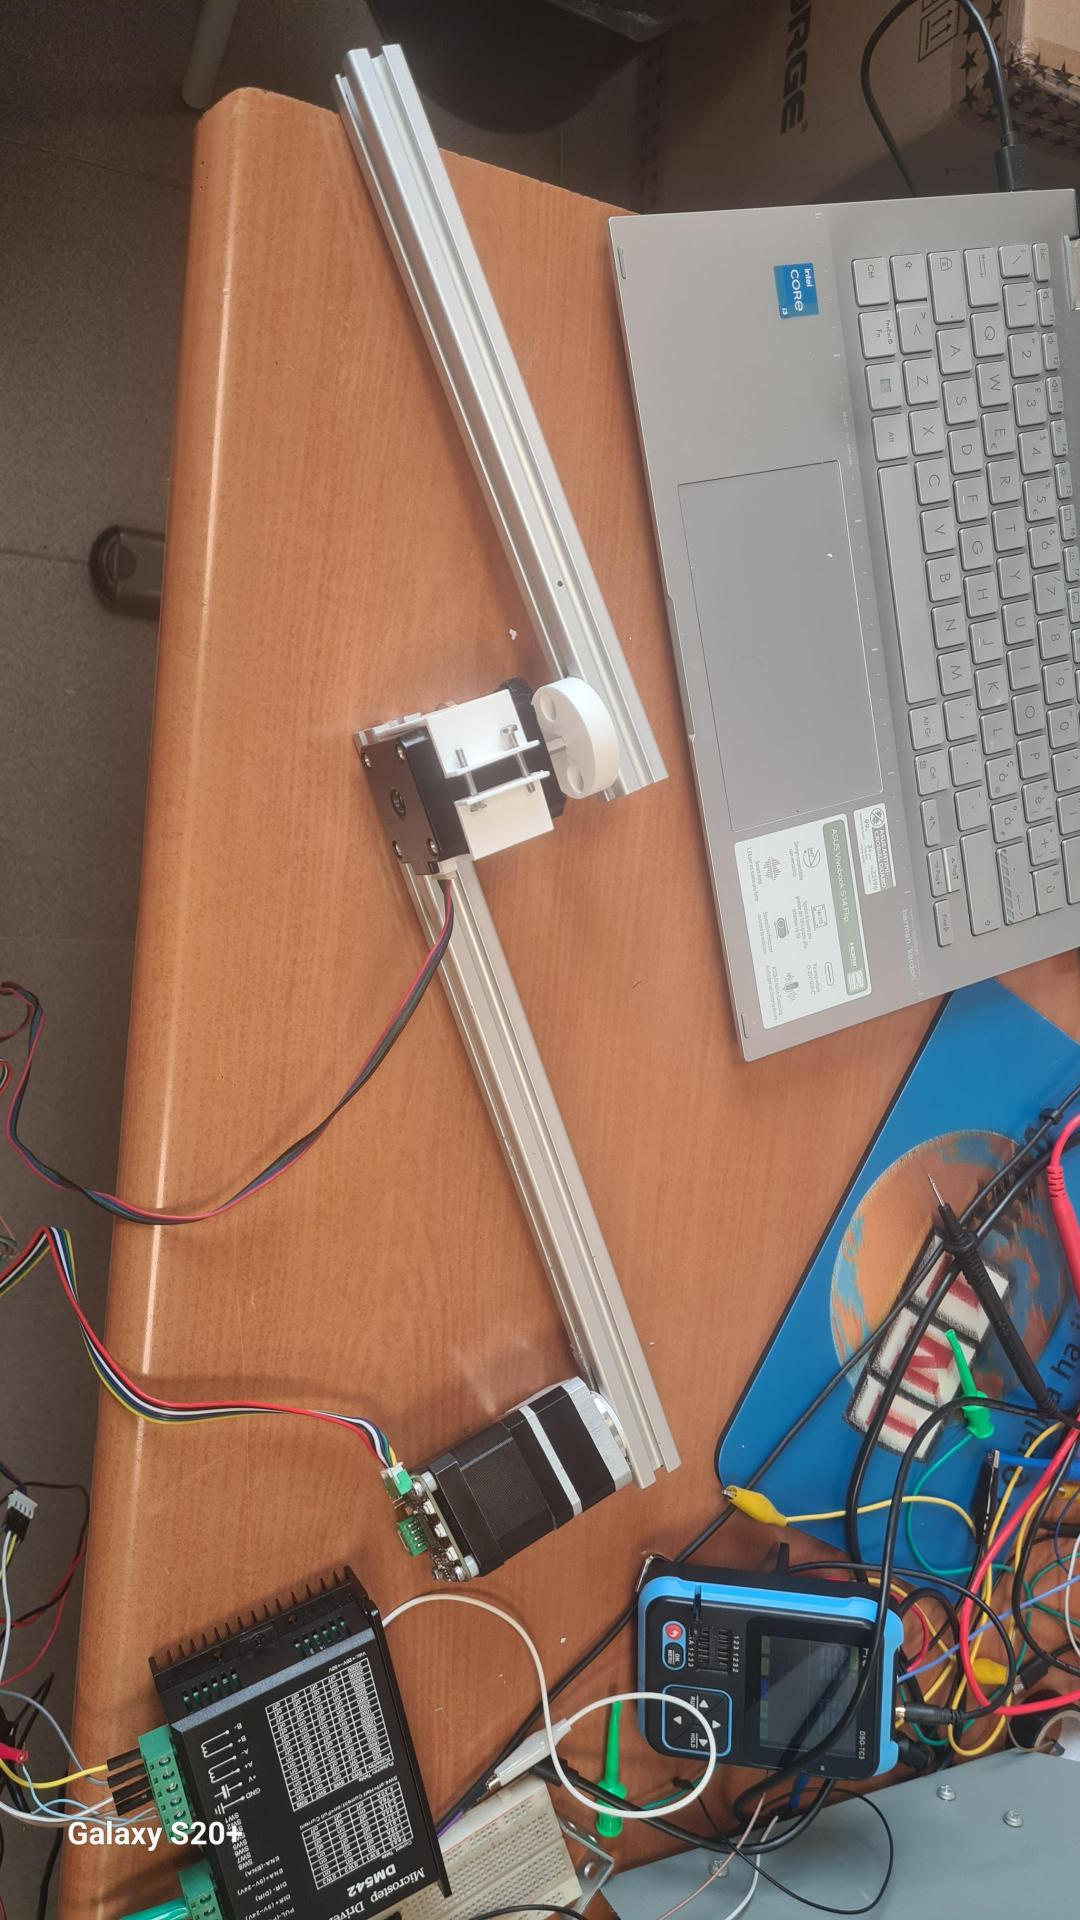
\includegraphics[width=0.7\linewidth]{\detokenize{pictures/semi assembled arm.jpeg}}
\caption{Bench test of the semi-assembled arm showing the base joint, shoulder link, stepper driver, and temporary wiring used for functional verification prior to full integration.}
\label{fig:semi_assembled_arm}
\end{figure}

The assembly sequence follows: (1) Base assembly with motor mounting and wiring, (2) Shoulder joint integration with gear reduction, (3) Forearm assembly with cable routing, (4) Wrist mechanism and end-effector mounting, (5) Electrical system integration and testing, (6) Final calibration and performance validation. Post-assembly calibration includes homing routine verification, limit-switch alignment, and zero-offset determination for each joint to establish a consistent reference frame for control and testing.

\section{Testing and Validation}

\subsection{Testing Protocol}
Comprehensive validation includes mechanical testing (static load testing for structural integrity under maximum payload, dynamic testing for motion smoothness and vibration analysis, repeatability testing for position accuracy over multiple cycles, endurance testing for long-term operation), electrical testing (power consumption analysis under various loads, signal integrity testing for communication reliability, safety system validation for emergency stop and limit switch functionality, control system testing for response time and accuracy), and integration testing (end-to-end functionality verification, software integration with control algorithms, performance benchmarking against design specifications, user acceptance testing for usability and reliability). Instrumentation may include encoders for joint position tracking, external motion capture or laser distance measurement for ground-truth accuracy, current sensing for driver characterization, and accelerometers for vibration assessment. Experimental sampling rates and trial counts are selected to ensure statistical significance and repeatability.

\subsection{Performance Analysis}
This subsection will present a comparative analysis of measured performance against the stated requirements, including accuracy, repeatability, payload capacity, and dynamic response. Results will be summarized with descriptive statistics and confidence intervals where appropriate, and discrepancies will be interpreted in light of modeling assumptions and manufacturing tolerances. The analysis will also identify predominant error sources (e.g., compliance, backlash, controller tuning) and propose targeted design or control refinements for subsequent iterations.

